\section{Lunghezza di un arco di curva}
La lunghezza di un arco regolare di curva $r(t)$, le cui equazioni parametriche sono date da 
    \begin{gather}
        x_i=x_i(t) \quad \text{con i = } 1,\dots , n \\ 
        \text{In un intervallo di tempo }t \in [a,b]
    \end{gather}
\subsection{Come la rappresento?}
Essa si rappresenta e si calcola attraverso un \textbf{integrale definito} compreso tra gli estremi $a$ e $b$ della curva.

L'operazione consiste \underline{nell'integrare la norma del vettore derivata della curva rispetto al tempo ($||\frac{dr}{dt}||$)}

\begin{definizione}{Forumla della Lunghezza di un arco di curva}
    $$ \LARGE
l = \int_{a}^{b} \sqrt{(\frac{dx_i}{dt})^2 + \dots + (\frac{dx_n}{dt})^2}
$$
\end{definizione}
\subsection{Esempio di calcolo}
Consideriamo un circonferenza nel Piano $\R^2$ con raggio $R$ costante
\begin{center}
    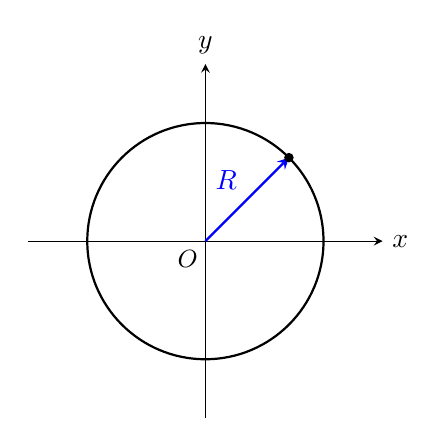
\begin{tikzpicture}[>=stealth, scale=1.5]
    % Assi
    \draw[->] (-1.5,0) -- (1.5,0) node[right] {$x$};
    \draw[->] (0,-1.5) -- (0,1.5) node[above] {$y$};
    
    % Circonferenza
    \draw[thick] (0,0) circle (1cm);
    
    % Raggio R
    \draw[->, blue, thick] (0,0) -- (45:1cm) node[midway, above left] {$R$};
    
    % Punto e origine
    \filldraw (45:1cm) circle (1pt);
    \node at (-0.15,-0.15) {\small $O$};
\end{tikzpicture}
\end{center}

La sua parametrizzazione standard è 
$
    r(t)=(R\cos(t),R\sin(t)) \quad \text{con }t \in [0,2\pi]
$ le componeneti sono quindi : 

$$
\begin{cases}
    x(t) = R\cos(t) \\ y(t)=R\sin(t)
\end{cases}
$$

Ora calcoliamo la norma del vettore derivata
\begin{gather}
    r(t)=
    \begin{bmatrix}
        R\cos(t) \\ R\sin(t)
    \end{bmatrix} 
    \implies r'(t) = 
    \begin{bmatrix}
        -R\sin(t) \\ Rcos(t)
    \end{bmatrix}\\
    ||r'(t)|| = \sqrt{(-R\sin(t))^2+(R\cos(t)^2)} = \sqrt{R^2(\sin^2(t)+\cos^2(t))} = \sqrt{R^2} = R
\end{gather}

\text{Ora inseriamo il risultato nell'integrale di linea per trovare la lunghezza }$l$
$$\LARGE
\int_a^b ||r'(t)||\, \mathrm{d}t = \int_{0}^{2\pi} R \, \mathrm{d}t = [R \cdot t]^{2\pi}_0 = R(2\pi - 0)=2\pi R
$$
\begin{center}
    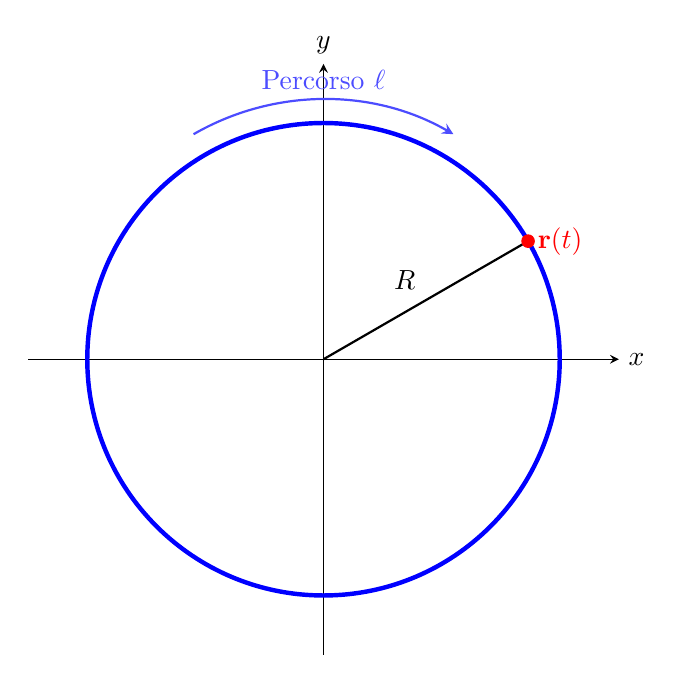
\begin{tikzpicture}[scale=1.5, >=stealth]
        % Assi coordinati chiari
        \draw[->] (-2.5,0) -- (2.5,0) node[right] {$x$};
        \draw[->] (0,-2.5) -- (0,2.5) node[above] {$y$};
        
        % La circonferenza (il cammino di integrazione gamma)
        \draw[ultra thick, blue] (0,0) circle (2);
        
        % Indicazione del raggio R
        \draw[thick] (0,0) -- (30:2) node[midway, above left] {$R$};
        
        % Punto generico e vettore r(t)
        \filldraw[red] (30:2) circle (1.5pt);
        \node[red, right] at (30:2) {$\mathbf{r}(t)$};
        
        % Freccia che indica lo sviluppo della lunghezza (Percorso l)
        \draw[->, thick, blue!70] (120:2.2) arc (120:60:2.2);
        \node[blue!70, above] at (90:2.2) {Percorso $\ell$};
        
        % NOTA: Il box "Risultato" è stato rimosso per pulizia
    \end{tikzpicture}
\end{center}

\newpage

\section{Integrali di linea di 1ª specie}
Data una funizione $f$ e una cruva regolare $C$ in $\R^n$, si inizia suddividendo la curva in piccoli archi di lunghezza $\Delta l$ e si sceglie un punto $P_i$ all'interno di ciascun arco.
\begin{center}
    \begin{definizione}{Formula integrale di linea di 1ª specie}
        $$
            \lim_{\|\Delta \ell\| \to 0} \sum_{i=1}^{n} f(P_i) \Delta \ell_i = \int_{C} f(x,y) \, ds
        $$
        \begin{itemize}
            \item $C$ : Rappresenta la \textbf{curva regolare} nello spazio lungo la quale si sta calcolando l'integrale
            \item $f$ : È la \textbf{funzione integranda}
            \item $\mathrm{d}\ell$ : È \textbf{l'elemento differenziale di lunghezza della curva}
            \item $t$ : È un \textbf{parametro arbitrario}
            \item $x_i(t)$ : Sono le \textbf{equazioni parametriche} della curva
        \end{itemize}
    \end{definizione}
\end{center}
\subsection{Come calcolarli?}
Per caloclare un integrale di linea di 1ª specie il metodo varia in base alla parametrizzazione della curva utilizzata
\subsubsection{Calcolo con parametri arbitrari}
Questa è la procedura pratica utilizzata quando la curva è descritta da un parametro generico $t$, basata sull'applicazione della formula di cambiamento di variabili

\vspace{\baselineskip}

Prendiamo come esempio l'integrale $\int_C xy^4 \, dl$ dove la curva $C$ è la semicirconferenza descritta dall'equazione $x^2+y^2=16$ posizionata nel semipiano $x \ge 0$
\begin{enumerate}
    \item \textbf{Parametrizzazione delal curva}
        \begin{itemize}
            \item \textbf{Procedura}

            Definire le equazioni parametriche $x(t),y(t)$ e l'intervallo degli estremi di integrazione
            \item \textbf{Calcolo}
            
            Poichè l'equazione $x^2+y^2=16$ descrive una circonferenza di raggio 4, e la limitazione è $x \ge 0$, la parametrizzazione usuale è 

            $$
                \begin{cases}
                    x(t)=4\cos(t) \\ y(t)=4\sin(t)
                \end{cases} \qquad t\in[-\frac{\pi}{2},\frac{\pi}{2}]
            $$

        \end{itemize}

    \item \textbf{Restrizione della funzione alla curva}

    Prendi la funzione integranda di partenza 
\end{enumerate}
\subsection{Esempio di calcolo con rappresentazione grafica}

